% !TEX root = ../YourName-Dissertation.tex

\chapter{Direct Measurement of the Neutrino Mass with Cyclotron Radiation Emission Spectroscopy}

\section{Introduction}

\section{Cyclotron Radiation Emission Spectroscopy}

Of the standard physical quantities the one that can be measured with the highest precision is time and the inversely related quantity frequency. In fact it is often advantageous to convert measurements of other physical quantities like mass or length into frequency measurements due to the digital nature of frequency measurements that make them immune to many sources of noise. Atomic clocks, which operate by measuring the frequencies of various atomic transitions, have been used to measure time with astounding relative uncertainties of $10^{-18}$~seconds. The extreme precision possible with frequency measurements is often summarized using the a quote from the Physicist Arthur Schawlow who said advise his students to "Never measure anything but frequency!". 

Neutrino mass measurements using tritium beta-decay are effectively attempting to measure  

\begin{figure}[htbp]
    \centering
    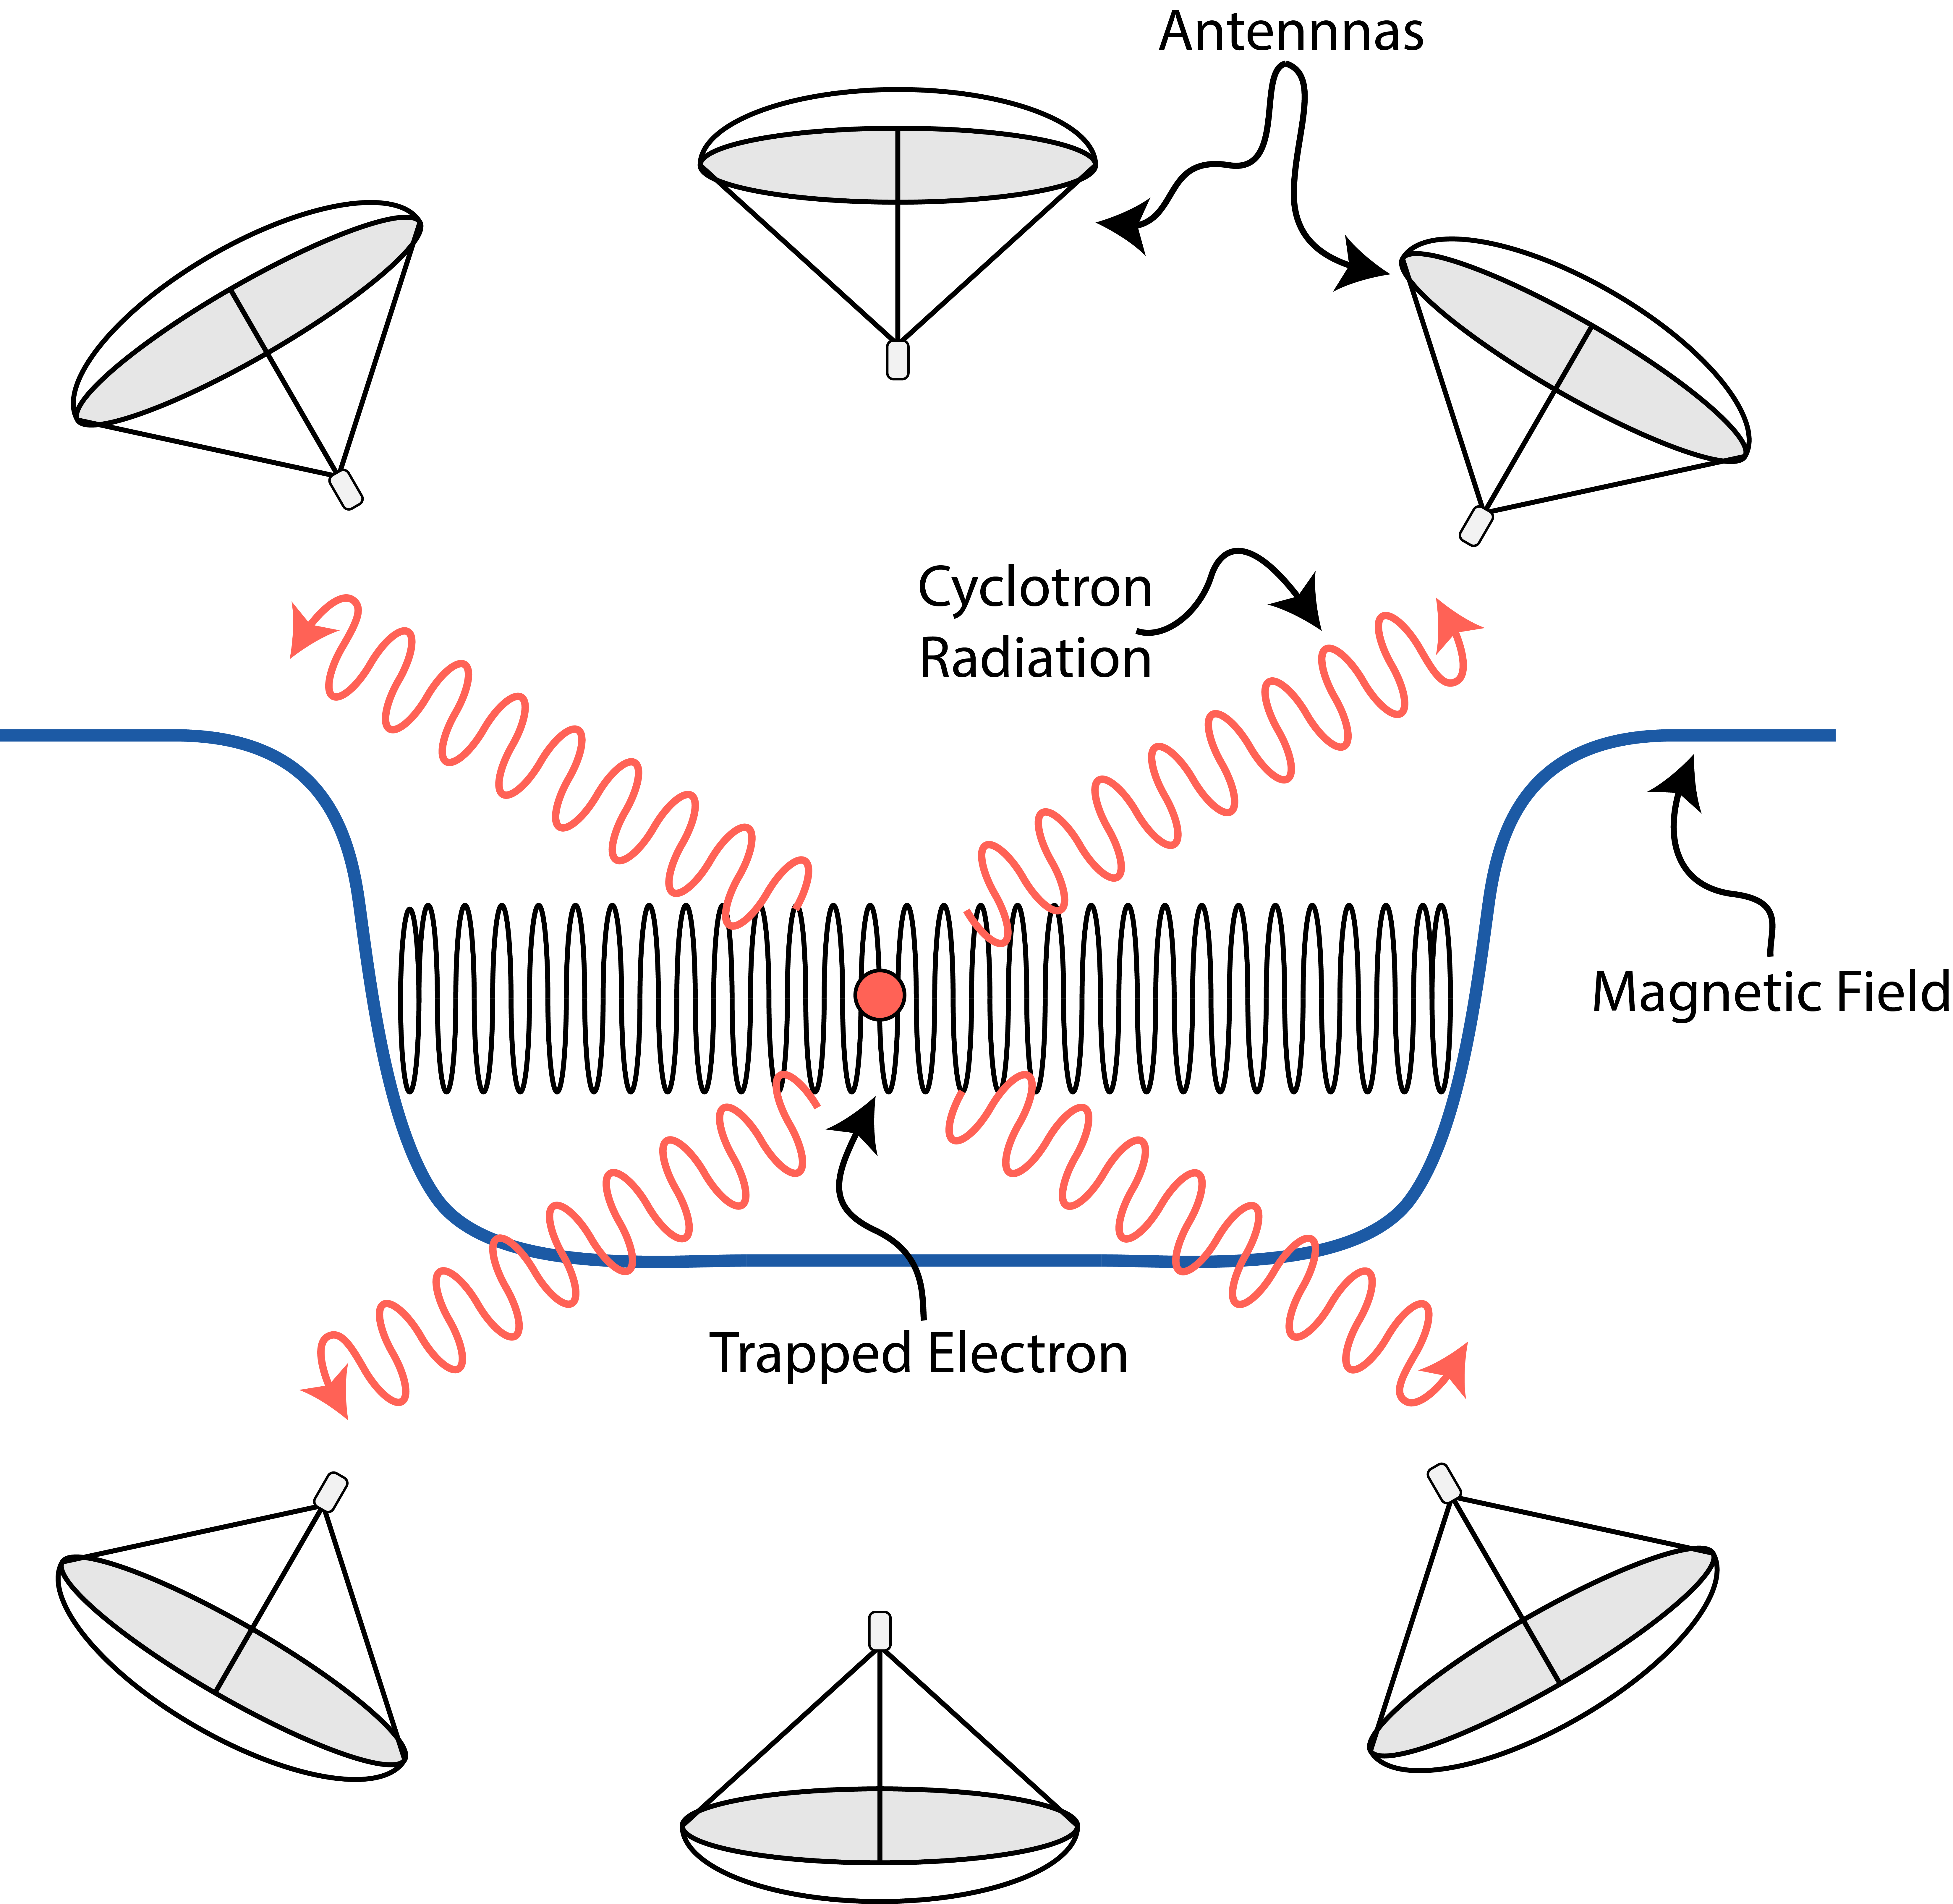
\includegraphics[width=0.5\textwidth]{figs/Chapter-3/230303_cres_cartoon.png}
    \caption{Caption}
    \label{fig:cres_cartoon}
\end{figure}

\subsection{Charged Particles in a Magnetic Trap}

\begin{figure}[htbp]
    \centering
    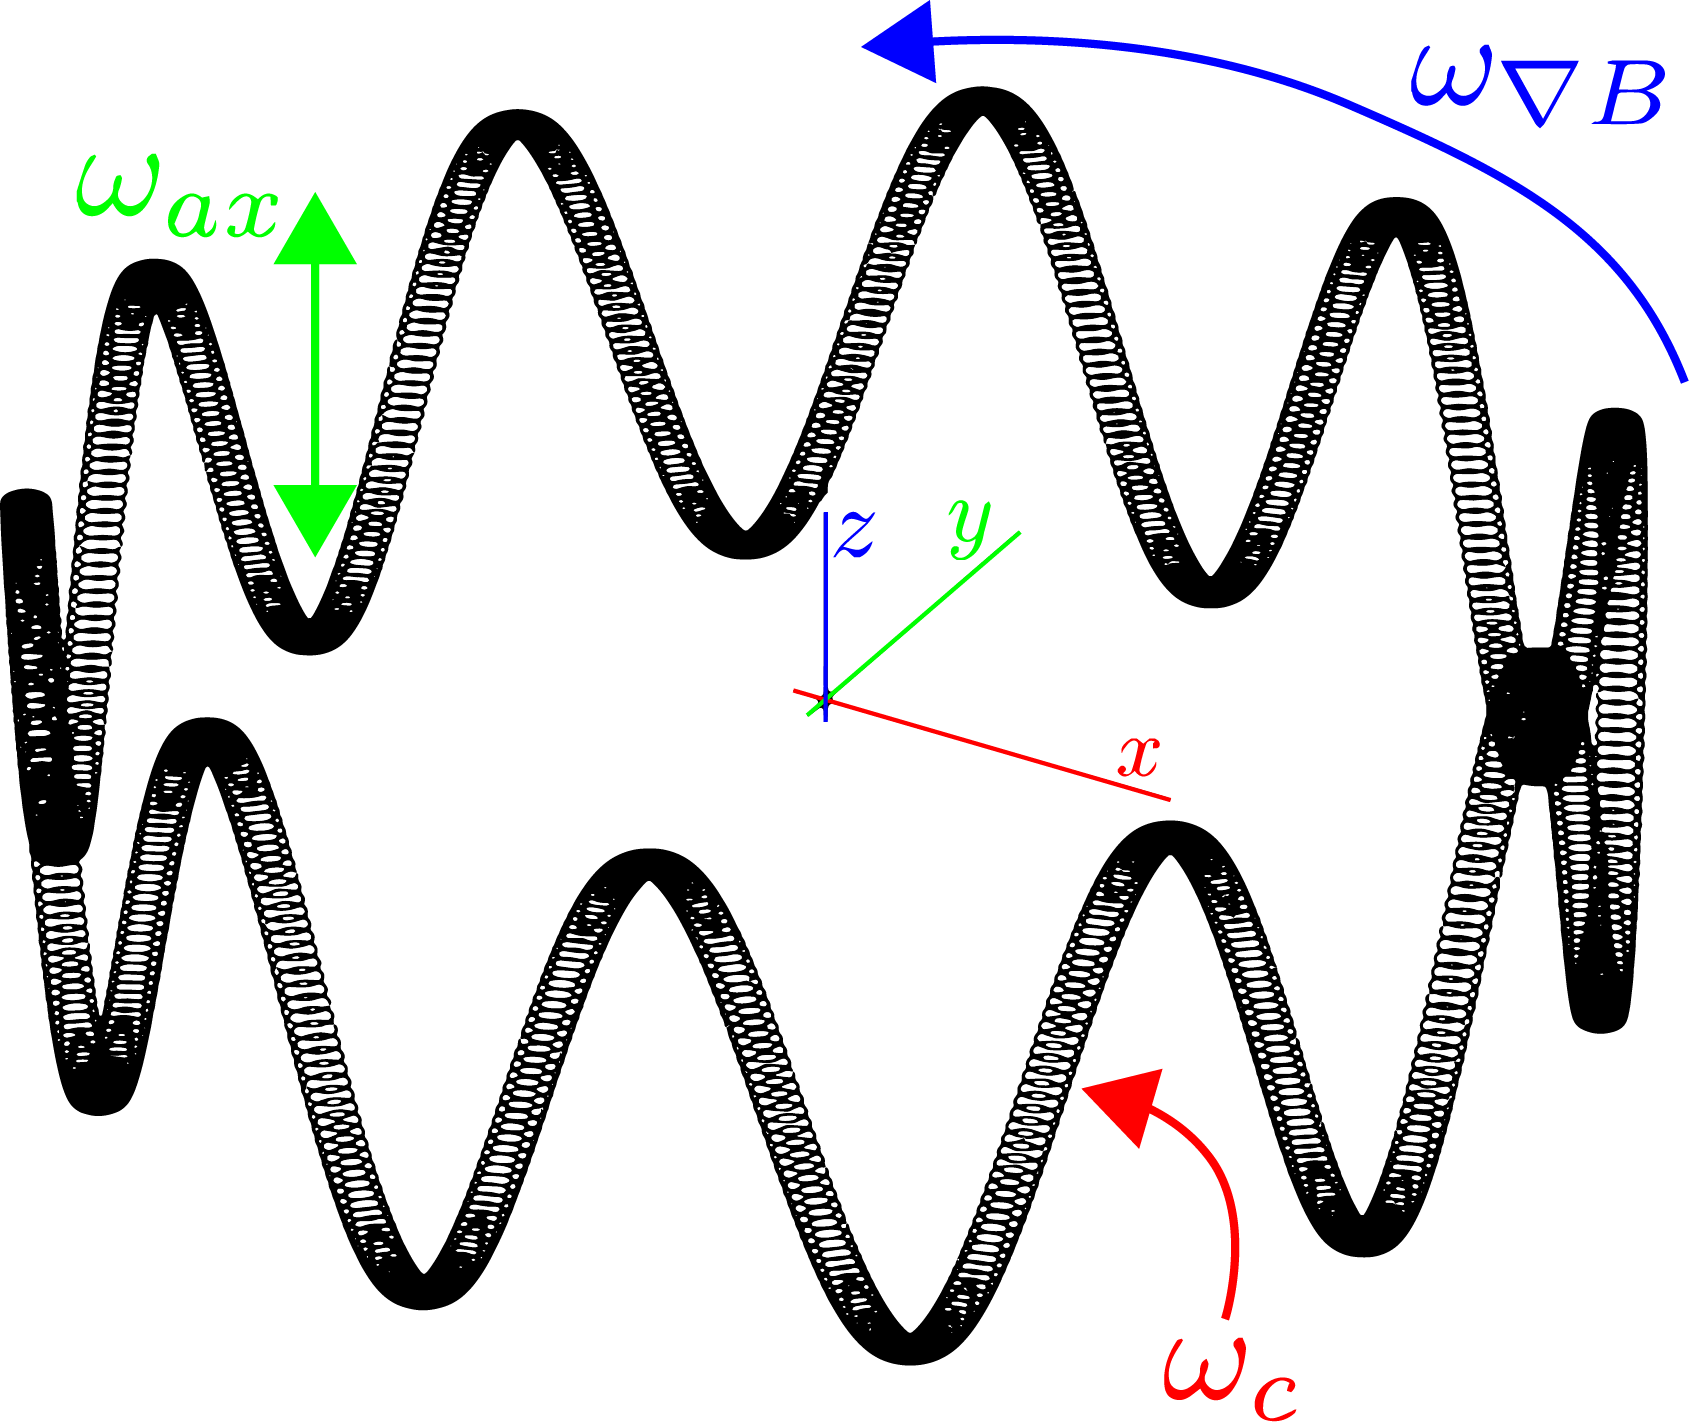
\includegraphics[width=0.5\textwidth]{figs/Chapter-3/230511_trapped_motion.png}
    \caption{Caption}
    \label{fig:chap3-trapped-electron-motion}
\end{figure}

\subsection{Radiation from a Charged Particle}

\section{The Project 8 Collaboration}

\subsection{Neutrino Mass Sensitivity Goals}

\subsection{Phased Development Plans}

\begin{figure}[htbp]
    \centering
    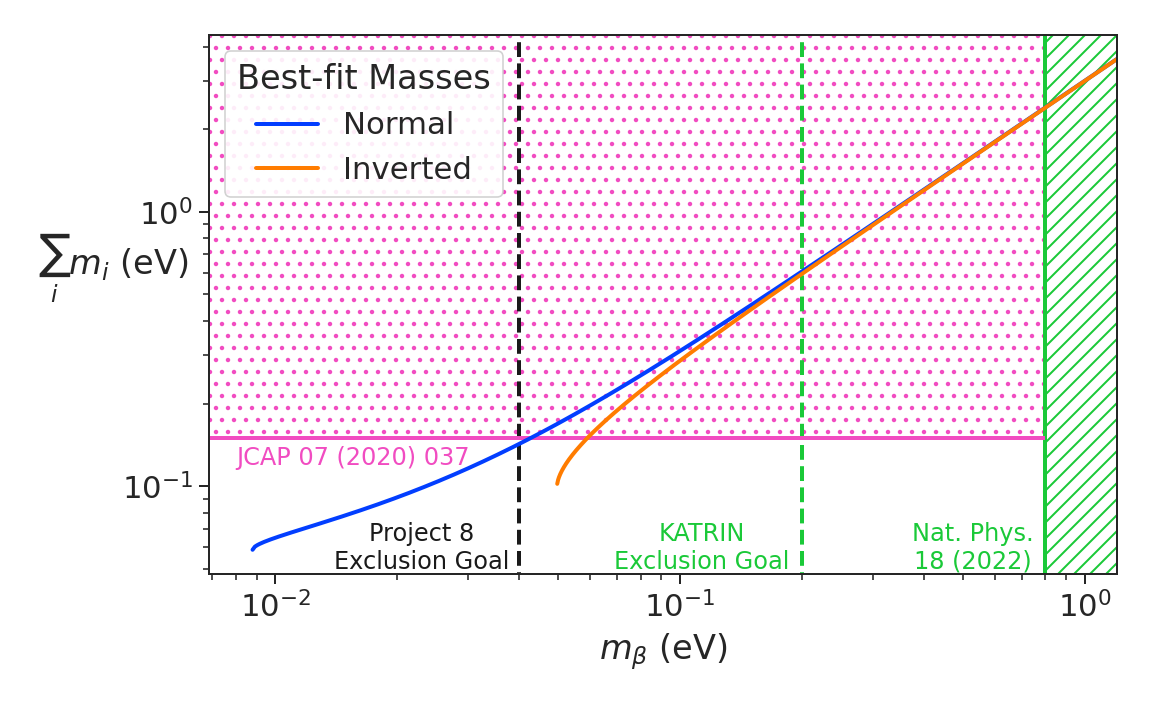
\includegraphics[width=0.7\textwidth]{figs/Chapter-3/230303_sum_nu_mass_vs_m_beta_with_exclusion_and_goal.png}
    \caption{Caption}
    \label{fig:p8_nu_mass_goal}
\end{figure}

\section{Phase II: First Tritium Beta Decay Spectrum and Neutrino Mass Measurement with CRES}

\subsection{The Project 8 CRES Demonstrator}

\begin{figure}[htbp]
    \centering
    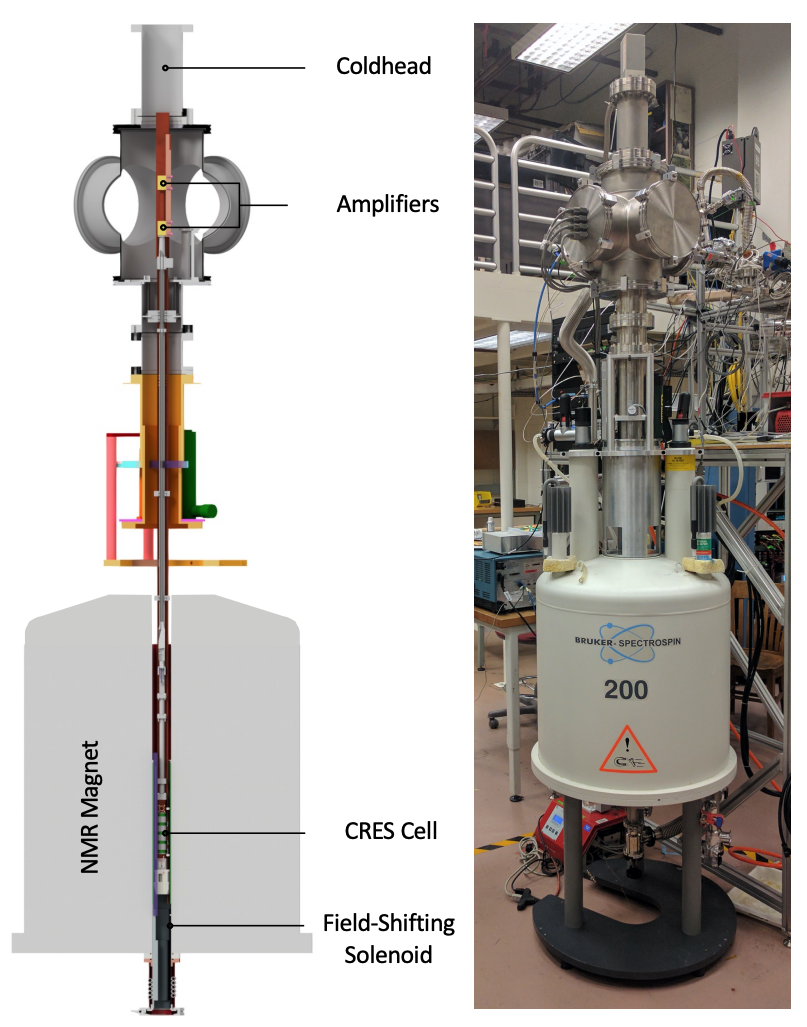
\includegraphics[width=0.7\textwidth]{figs/Chapter-3/phaseII_system.png}
    \caption{Caption}
    \label{fig:phase2_apparatus}
\end{figure}

\begin{figure}[htbp]
    \centering
    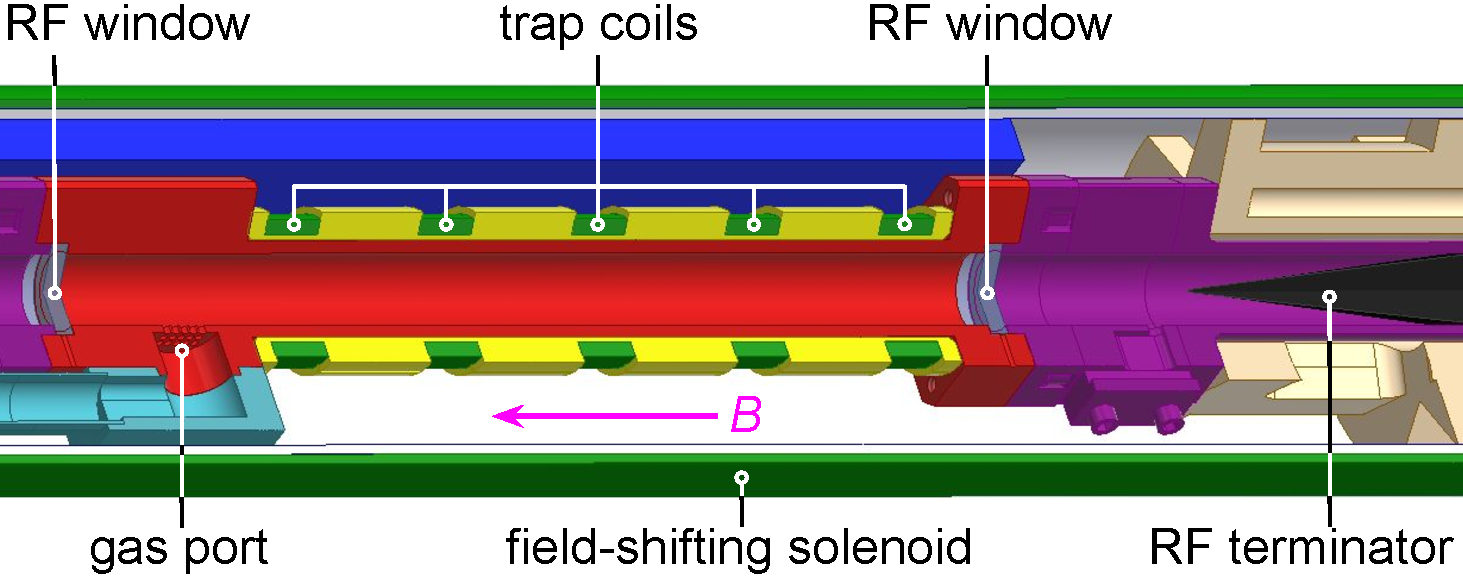
\includegraphics[width=0.8\textwidth]{figs/Chapter-3/apparatus.pdf}
    \caption{Caption}
    \label{fig:phase2_cres_cell}
\end{figure}

\subsection{CRES Track and Event Reconstruction}

\begin{figure}[htbp]
    \centering
    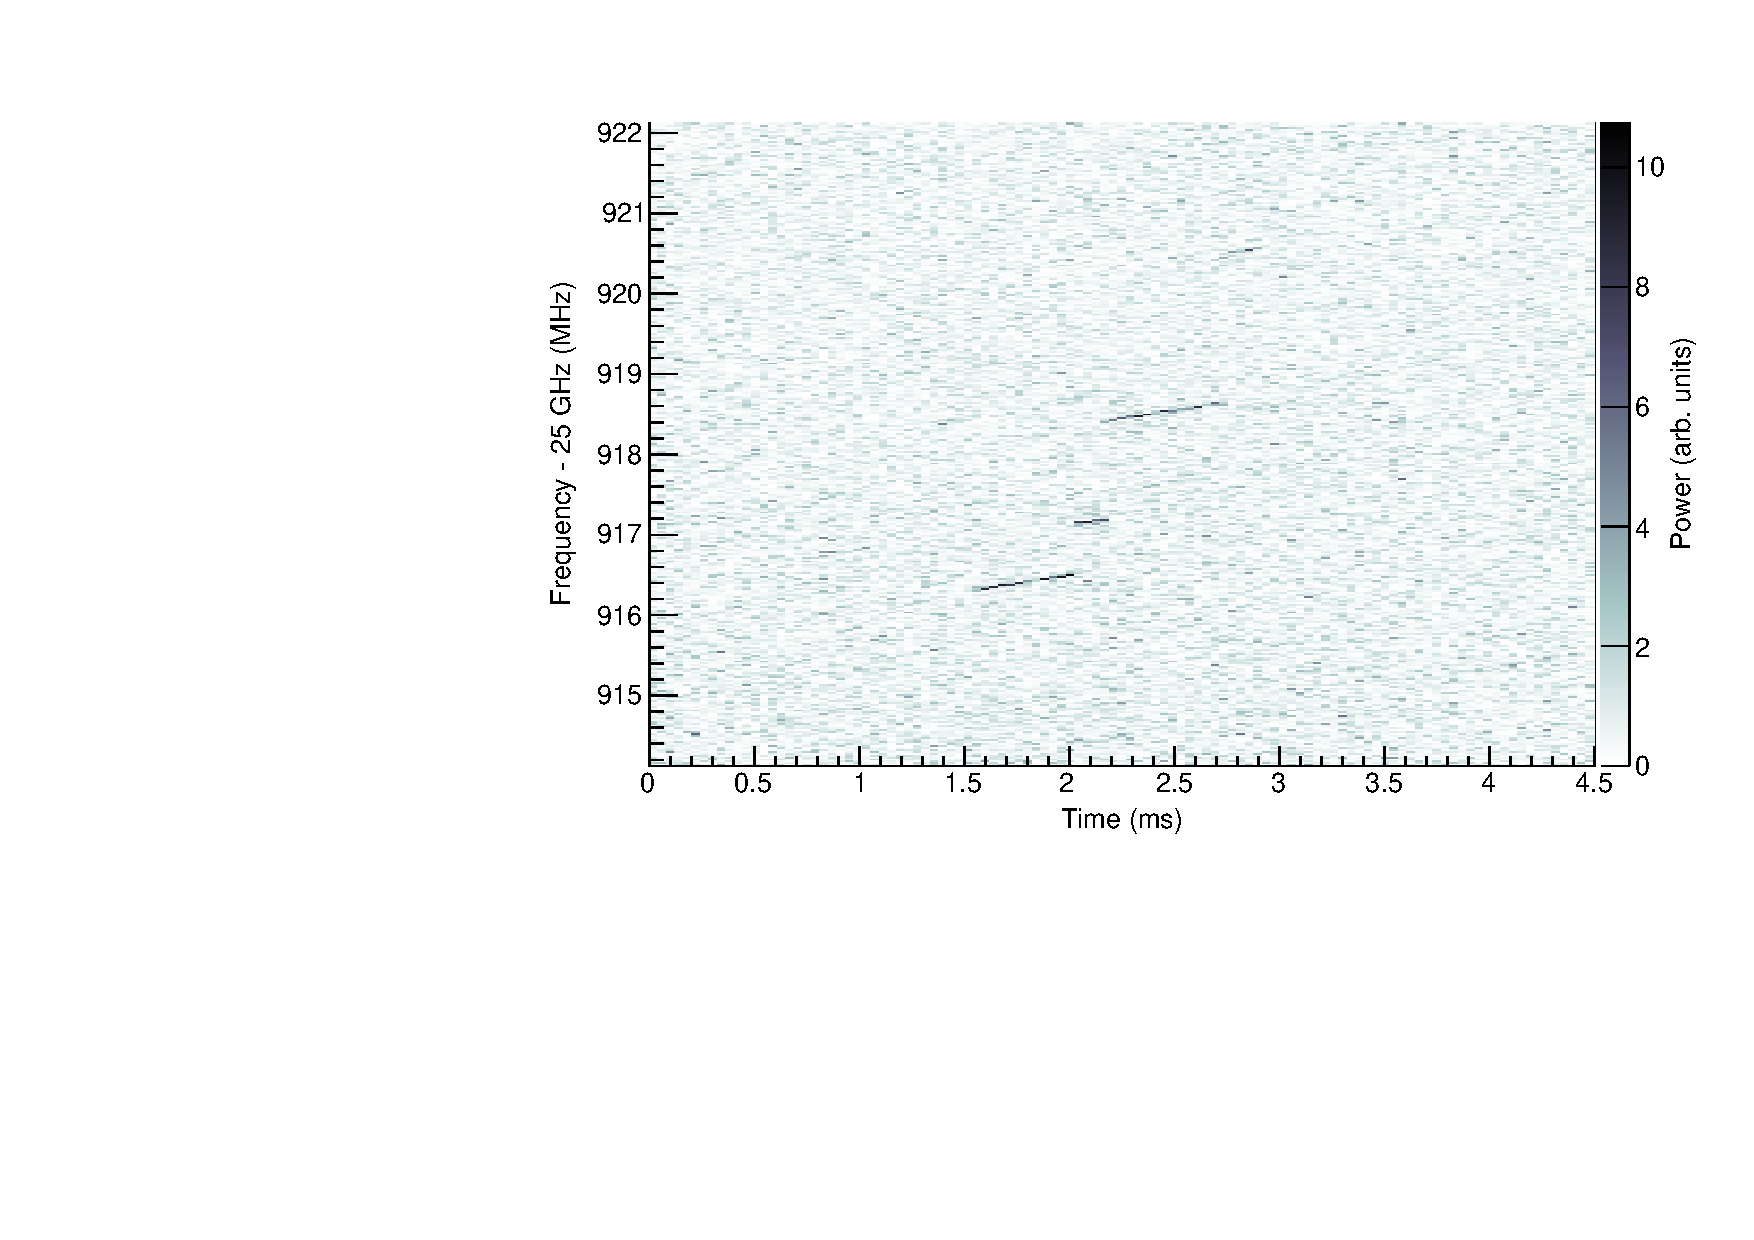
\includegraphics[width=0.7\textwidth]{figs/Chapter-3/T2_Event0.pdf}
    \caption{Caption}
    \label{fig:tritium_event0}
\end{figure}

\subsection{Measurements with Krypton}

\begin{figure}[htbp]
    \centering
    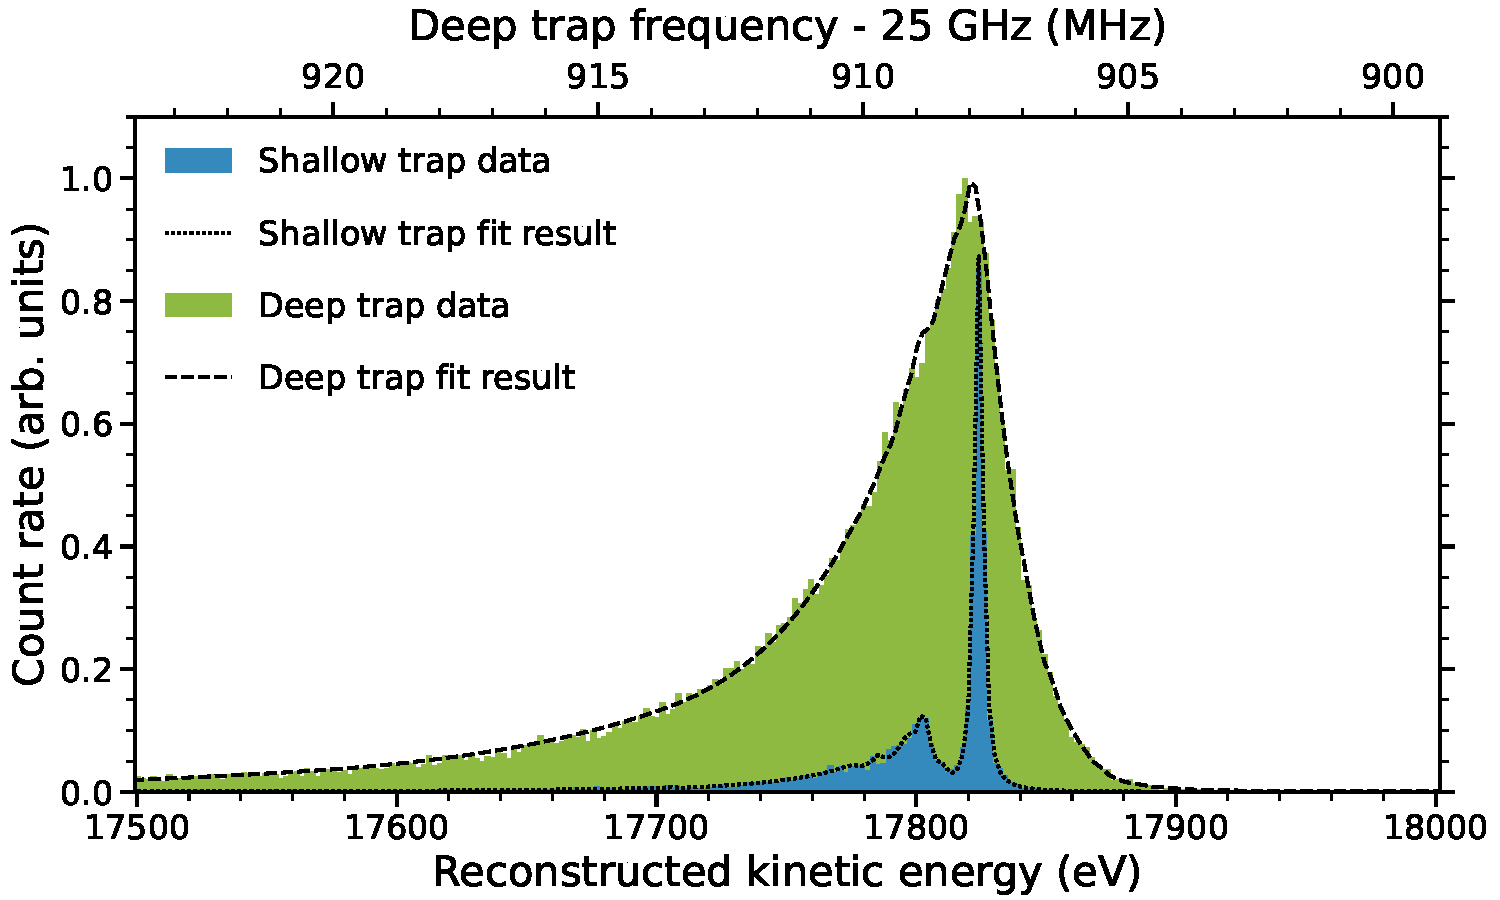
\includegraphics[width=0.7\textwidth]{figs/Chapter-3/kr_fit.pdf}
    \caption{Caption}
    \label{fig:krypton_fit}
\end{figure}

\begin{figure}[htbp]
    \centering
    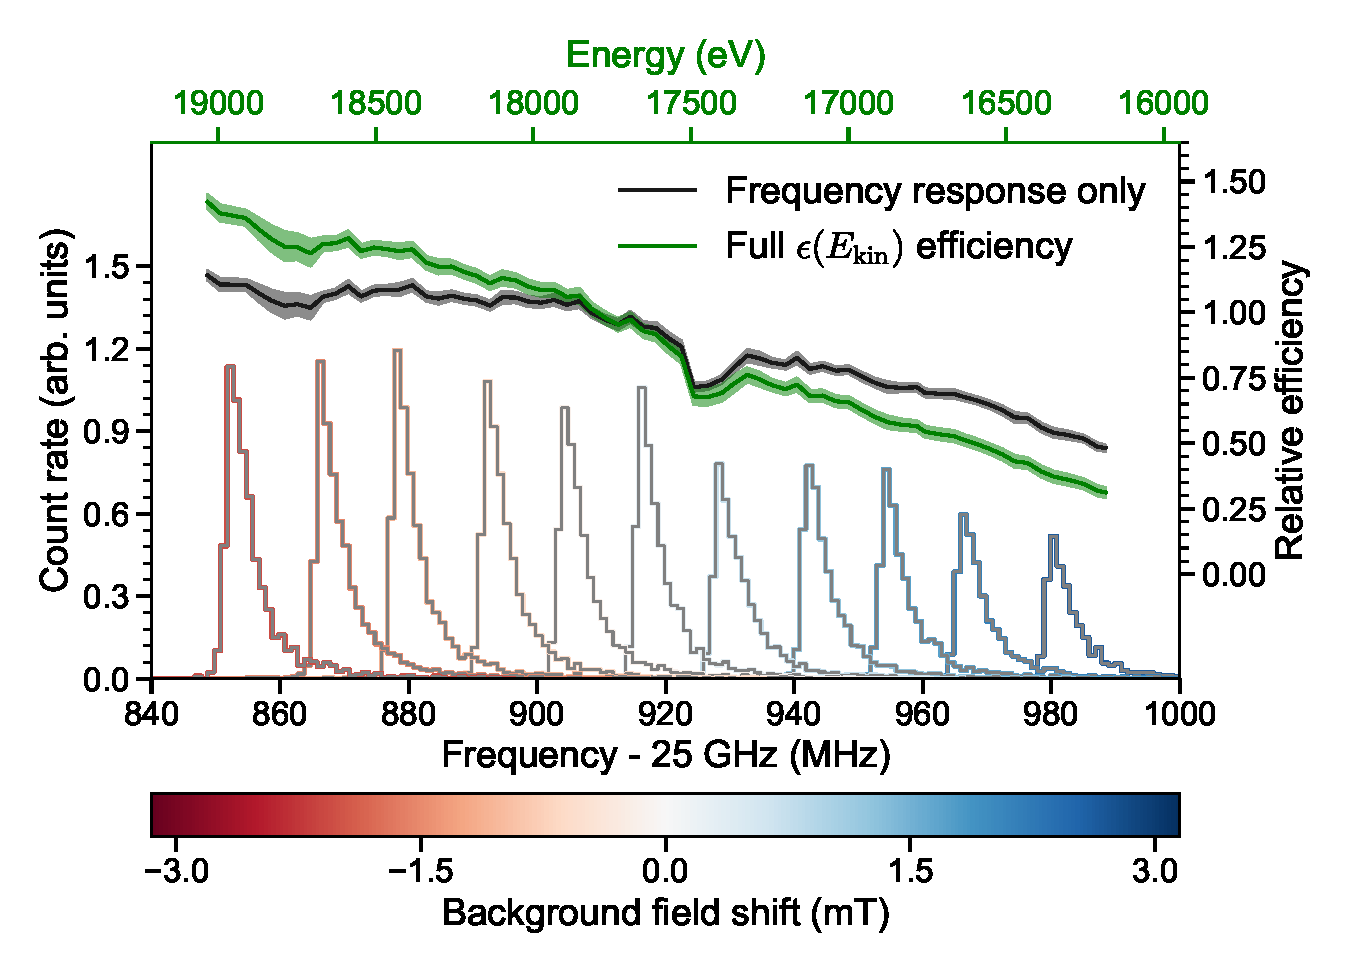
\includegraphics[width=0.7\textwidth]{figs/Chapter-3/fss_for_prl_plot.pdf}
    \caption{Caption}
    \label{fig:fss_plot}
\end{figure}

\subsection{Tritium Spectrum and Neutrino Mass Results}

\begin{figure}
    \centering
    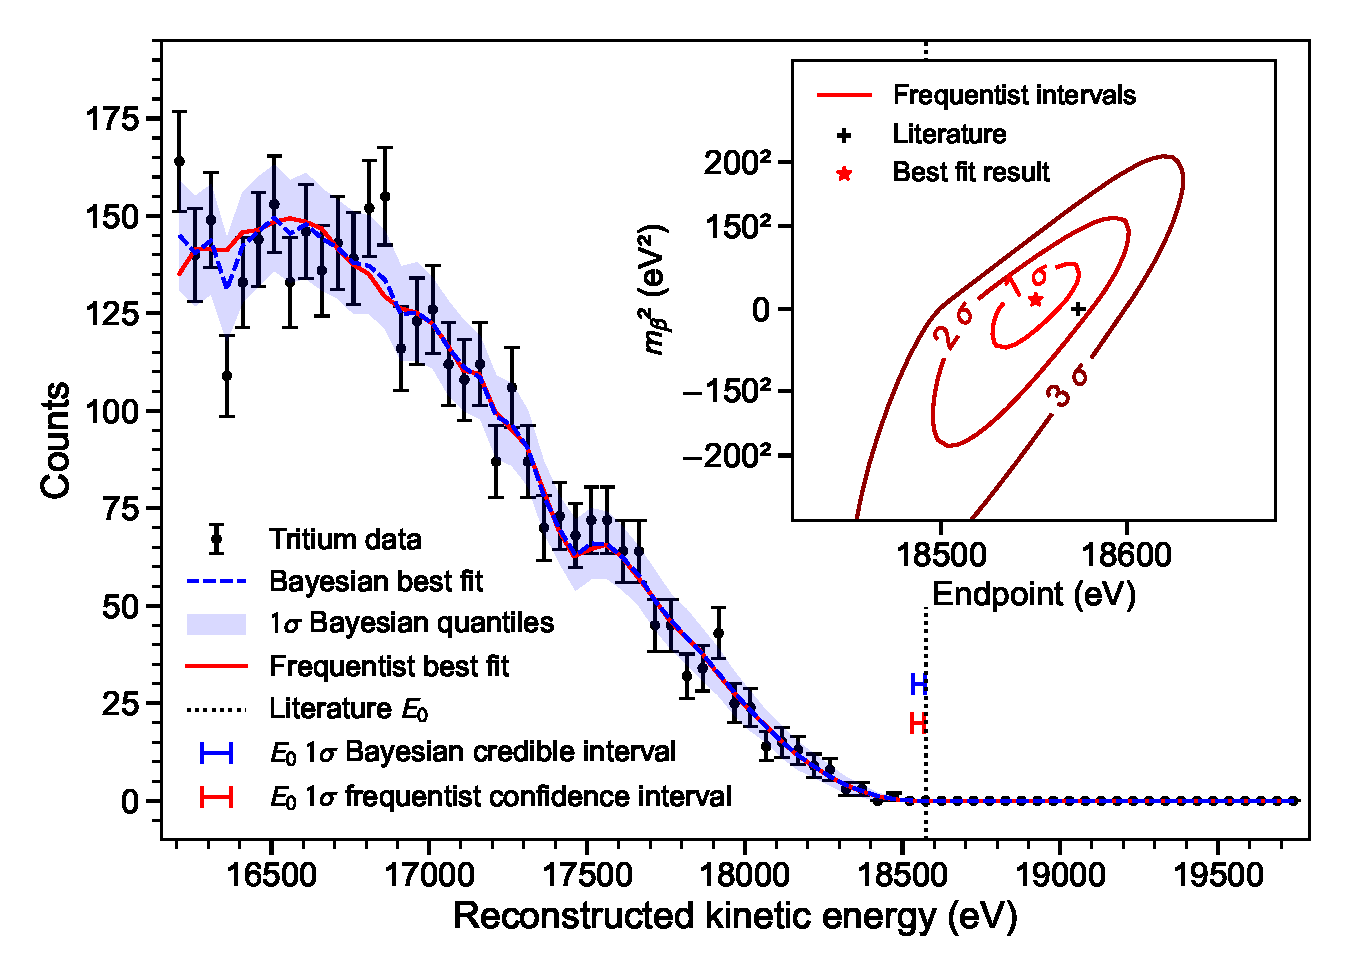
\includegraphics[width=0.7\textwidth]{figs/Chapter-3/12-03-22A_final_E0_real_data_phase_II_tritium_fit_1d.pdf}
    \caption{Caption}
    \label{fig:final_tritium_fit}
\end{figure}

\section{Phase III: Developing Free-space CRES Measurements with Antenna Arrays}

The goal of Phase III in the Project 8 experimental program is to develop the technologies and expertise required to build an experiment that uses CRES to measure the neutrino mass with a target sensitivity of 40~meV. One of the key technologies is a method for performing high resolution CRES measurements in a large volume, which allows one to observe a sufficient quantity of tritium to measure the low-activity endpoint region of the tritium spectrum. 

\subsection{The Basic Approach}

One possible approach, suggested in the original CRES publication, is to use many antennas to surround a volume of tritium gas in a magnetic field (see Figure \ref{fig:chap3-antenna-concept-cartoon}). When a decay occurs the electron will begin to emit cyclotron radiation that can be collected by the array and used to perform CRES. 
\begin{figure}[htbp]
    \centering
    \includegraphics*[width=0.6\textwidth]{figs/Chapter-3/230614_antenna_cartoon.png}
    \caption{\label{fig:chap3-antenna-concept-cartoon}}
\end{figure}
Scaling to large volumes with the antenna array approach is accomplished by increasing the number of antennas in the array, which increases the volume under observation proportionally. 

Several features of the antenna array approach make it an attractive candidate technology for a large volume experiment. One example is the accurate position reconstruction made possible by the multichannel nature of the array. Using techniques like digital beamforming it is possible to estimate the radial and azimuthal positions of the electron in the magnetic trap with a precision significantly less than the size of the cyclotron wavelength. This capability allows one to perform event-by-event estimations of the magnetic field experienced by an electron, which is crucial to achieving high energy resolution with the CRES technique. 




\subsection{The FSCD: Free Space CRES Demonstrator}

\subsubsection*{Magnetic Field}

\begin{figure}[htbp]
    \centering
    \includegraphics*[width=0.5\textwidth]{figs/Chapter-3/230614_mri_magnet.png}
    \caption{}
\end{figure}

\subsubsection*{Gas System and Tritium Source}
\subsubsection*{Antenna Array}

\begin{figure}[htbp]
    \centering
    \includegraphics*[width=0.4\textwidth]{figs/Chapter-3/230614_5slot_model.png}
    \caption{}
\end{figure}

\begin{figure}[htbp]
    \centering
    \includegraphics*[width=0.7\textwidth]{figs/Chapter-3/230614_fscd_render.png}
    \caption{}
\end{figure}

\subsubsection*{Scaling}

\begin{figure}[htbp]
    \centering
    \includegraphics*[width=1\textwidth]{figs/Chapter-3/230614_large_scale_antenna.png}
    \caption{}
\end{figure}


